\documentclass[11pt]{article}

% Basic packages
\usepackage{amsmath}
\usepackage{graphicx}
\usepackage{parskip}
\usepackage[section]{placeins}
\usepackage[capitalise, noabbrev]{cleveref}
\usepackage{csvsimple}
\usepackage{booktabs}
\usepackage[margin=3cm]{geometry}
\usepackage[table,xcdraw]{xcolor}
\usepackage{tikz}
\usetikzlibrary{math,calc,positioning}

\usepackage[backend=biber]{biblatex}
\bibliography{bibliography}

\usepackage{todonotes}

% Set up fonts
\usepackage{fontspec}
\usepackage{unicode-math}
\setmainfont{STIX Two Text}
\setmathfont{STIX Two Math}

\title{IN5410 - Assignment 2}
\author{David Andreas Bordvik, Koen van Greevenbroek, Taeo Laue}
\date{\today}

\begin{document}

\maketitle

\section*{Question 1}
% \subsection*{Introduction}
The main goal for this task is to predict wind power generation in November 2013 using historical data and different types of machine learning methods. The target variable specified for this task is wind power generation, and we are told to use wind speed 10 meters above the ground as our single feature in the input data for the machine learning model.

In machine learning (ML), the main idea is to create a model that can learn to map input data to outputs. The training process of an ML model results in a model that is fitted to memorize patterns within the data while incorporating relationships between different features. This assignment is based on the supervised learning paradigm, a sub-category out of the four main ML categories; supervised learning, unsupervised learning, semi-supervised learning, and reinforcement learning. Supervised learning relies on the model having access to a target variable during training. For this task, we are given the target variable for power production, which is a continuous target variable. Since the target for the training data is numerical and continuous, and the model's outcome is expected to be continuous, we have a regression problem. Furthermore, the assignment expects a comparison of three classical ML models and one deep learning model. Deep learning is regarded as a subset of machine learning. Deep learning utilizes artificial neural networks (ANN) that mimic the human brain through a set of advanced algorithms. 


\subsection*{The problem}
As mentioned in the above, we face a regression problem using supervised learning, both for the deep learning model and the three classical ML approaches. We consider the problem of predicting wind farm power output based on wind speed.
Let $s$ be wind speed\footnote{Units are nowhere specified, but we presume meters per second.}, and let $p$ be power output\footnote{In watts, but normalised by some unknown amount.}. In ML we assume that there is some unknown function $f$ such that
\begin{equation*}
  p = f(s).
\end{equation*}
We have access to training data in the form of a number of observations $(p_i, s_i)$ such that $p_i = f(s_i)$.
Our task is to use the training data to find an approximation $\hat{f}$ of $f$.
The approximation enables us to estimate $p = f(s)$ by $\hat{p} = \hat{f}(s)$ for previously unseen values of $s$.
A good approximation $\hat{f}$ should give small differences between $p = f(s)$ and $\hat{p} = \hat{f}(s)$.
We use the root-mean-square error (RMSE) to compute the difference between $f$ and $\hat{f}$ over a set of testing data; measurements for November 2013 in our case.
Let $(p_i, s_i)$ for $i \in N$ be test data for November (which was not used as training data for $\hat{f}$).
Then the RMSE between $\hat{f}$ and $f$ is defined as
\begin{equation*}
  \sqrt{\frac{1}{|N|} \sum_{i \in N} \left(\hat{f}(s_i) - p_i\right)^2}.
\end{equation*}

Additionally we want to compare different approaches for predicting $f$.
Some of the approaches (e.g.\ linear regression) give a closed-form expression for $\hat{f}$ while others (e.g.\ nearest-neighbour, neural networks) result in algorithms for computing $\hat{f}$.
We evaluate the effectiveness of each model using the RMSE as discussed above; closer to $0$ is better.
For the artificial neural network model in particular, we also evaluate whether the model may have over-fitted the training data.

% During training, we have access to the true target variable $p$. Performing inference using a trained model on new previously unseen data, the true target variable $p$ is no longer known. However, we can assume that the model predicts $\hat{p}$ not too far from the theoretical true value of the unknown $p$. Optimally the residual deviance between $\hat{p}$ and $p$ should look similar to what can be achieved performing inference on the data the model has been trained on where the true values for $p$ are known. 

% Furthermore, for the ANN model, the assumption above implies that the model is not overfitted or underfitted to the training data, and that the model has been generalized properly during the training process.


\subsection*{Input data and data analysis}
One of the most important aspects of ML is the quality of the data. For our case, we expect that there is a relationship between wind speed $s$ and the actual generated power $p$, given by $f$. 
% The input data must therefore incorporate information influencing the outcome such that the model can learn their relationship. 
However, it's highly likely that other factors besides wind speed at 10m also affect the amount of generated power.
Therefore, we don't expect a ``perfect'' relationship between wind speed and generated power.
Specifically, for any function $f$ depending only on wind speed, the generated power $p$ with a wind speed of $s$ is \emph{close} to $f(s)$, but not always exactly equal.
In other words, even the unknown function $f$ which we want to approximate probably has a non-zero RMSE on the testing data.
This also makes it unlikely for any estimation $\hat{f}$ to achieve a RMSE very close to 0.

The training data we use, contained in the \texttt{TrainData.csv} file, consists of time series data including measurements of wind speed $s$ and power output $p$.
The data consists of hourly measurements from 01.01.2012 to 31.10.2013.
In fact, in addition to the wind speed we are also given the wind speed components in the $x$ and $y$ directions, effectively giving us the wind angle.
This is used in the next question.
Additionally, we have all of the above data measured at two different altitudes: 10 meters and 100 meters.
For this assignment, we only use the measurements taken at 10 meters.

To get some quick intuition about the data, consider the correlation matrix between the different columns in \texttt{TrainData.csv}, in \cref{fig:q1-corr-analysis}.
The most important part of the matrix is the POWER row, showing the correlation between this and the other columns.
We can see that there is a good correlation between POWER and WS10 (the wind speed at 10 meters altitude), which is the parameter we are using.
The correlation with WS100, the wind speed at 100 meters altitude, is even higher, suggesting that this would also be a useful parameter.

\begin{figure}
  \centering
  \includegraphics{figures/q1_corr_analysis.pdf}
  \caption{Correlation analysis of columns in \texttt{TrainData.csv}.}
  \label{fig:q1-corr-analysis}
\end{figure}

A high correlation shows a near-linear relationship between two parameters.
This suggests that a linear regression approximation for $f$ should already be quite effective.
Hopefully, more sophisticated methods should give an even higher degree of accuracy than linear regression.

Once we have trained different models on the training data, we use them to predict power output for a new period.
In particular, we have one month (November 2013) of wind speed measurements in the same format as the training data, found in \texttt{WeatherForecastInput.csv}.
Our task is to ``predict'' power output for November 2013 using these measurements.
For testing purposes, we also have the complete measurements (including power data) for November 2013 in \texttt{Solution.csv}.
As previously discussed, we compute the RMSE between the predicted power output and the real data given in \texttt{Solution.csv} in order to evaluate the different models.

\subsection*{Model setup and approach}

We use four different regression models to predict wind power output:
\begin{enumerate}
\item
  Linear regression.
\item
  $k$-Nearest Neighbour (kNN).
\item
  Support Vector Regression (SVR).
\item
  Artificial Neural Network (ANN).
\end{enumerate}

The application of these models is mostly straight-forward, and we refer directly to the attached code for implementation details.
However, for some of the models there are hyperparameters and other choices to discuss.
Short of a rigorous hyperparameter optimisation such as a grid-search, finding the right hyperparameters for particular problems usually involves some experimentation.
In our case, informal experimentation is sufficient as we don't have to deal with many hyperparameters.

There are no hyperparameters for linear regression.

For the $k$-Nearest Neighbour model, we need to choose a value for $k$.
Because we have relatively large amount of training data ($\approx 16000$ points) within a relatively small interval (wind speeds between 0 and 15), we chose a rather large value for $k$.
After some experimentation, the model seems quite insensitive to the value of $k$ in the order of magnitude $[300, 3000]$; we chose $k=1000$.

We use a Support Vector Regression model using the kernel trick, with the Radial Basis Function (RBF) as a kernel function.
This is a standard, flexible kernel function which allows us to fit non-linear data.
Apart from the kernel function, we need to choose the regularization parameter $C$ and the allowed error $\epsilon$.
The parameter $\epsilon$ determines the width of the band around the predicted regression within which the loss function for training data is set to $0$.
Data outside the $\epsilon$-wide band is weighed proportional to $C$ in the loss function (the other component in the loss function being the norm of the vector $\mathbf{w}$ determining the direction of the predicted hyperplane in the kernel space).
In our case, we left $C$ at the default of $1$.
After some experimentation, we set $\epsilon = 0.05$. Values in the range of $[0.01, 0.15]$ give a good RMSE on the testing data, but lower values of $\epsilon$ predict highs and lows in power output better.

The most choice is involved in constructing an artificial neural network for the regression problem.
There are a number of factors to consider: the number of layers in the network, the number of nodes in each layer, the activation function of the nodes and parameters related to the training of the network.
A structural hyperparameter optimisation is out of the scope of this assignment, so we have made choices based on simple guidelines, which seem to produce good results.

In our case, we are approximating a simple function from $\mathbb{R}$ to $\mathbb{R}$ (i.e.\ in only one parameter) with little variation over its domain.
This warrants a simple design.
The architecture of our neural network is as illustrated in \cref{fig:ANN}, except that we use 15 nodes in the hidden layer.
We used the $\tanh$ function as the activation function for all the hidden neurons, and a linear activation function for the output node.
For the training, we used a typical setup: a stochastic gradient descent (implemented in Tensorflow as the ``Adam'' optimiser) with a learning rate of $0.001$ and 50 epochs.
After some experimentation, we found that the above parameters give good results.

\begin{figure}
  \centering
  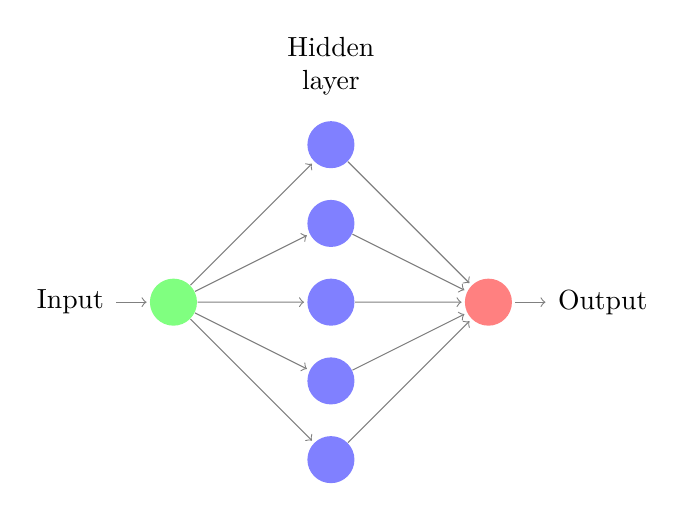
\begin{tikzpicture}[shorten >=1pt,->,draw=black!50, node distance=\layersep]
    \tikzstyle{every pin edge}=[<-,shorten <=1pt];
    \tikzstyle{neuron}=[circle,fill=black!25,minimum size=17pt,inner sep=0pt];
    \tikzstyle{input neuron}=[neuron, fill=green!50];
    \tikzstyle{output neuron}=[neuron, fill=red!50];
    \tikzstyle{hidden neuron}=[neuron, fill=blue!50];
    \tikzstyle{annot} = [text width=4em, text centered];
    \tikzmath{
      \nhidden = 5;
      \layersep = 2;
    }

    % Draw the input layer node
    \node[input neuron, pin=left:Input] (I) at (0,-\nhidden/2) {};

    % Draw the hidden layer nodes
    \foreach \name / \y in {1,...,\nhidden}
    \path[yshift=0.5cm]
    node[hidden neuron] (H-\name) at (\layersep,-\y cm) {};

    % Draw the output layer node
    \node[output neuron,pin={[pin edge={->}]right:Output}] (O) at (2*\layersep, -\nhidden/2) {};

    % Connect every node in the input layer with every node in the
    % hidden layer.
    \foreach \dest in {1,...,\nhidden}
    \path (I) edge (H-\dest);

    % Connect every node in the hidden layer with the output layer
    \foreach \source in {1,...,\nhidden}
    \path (H-\source) edge (O);

    % Annotate the layers
    \node[annot,above of=H-1, node distance=1cm] (hl) {Hidden layer};
  \end{tikzpicture}
  \caption{An illustration of the type of artificial neural network used for regression. Note our model was constructed with 15 nodes in the hidden layer.}
  \label{fig:ANN}
\end{figure}

One aspect to keep in mind when designing a neural network is to limit the number of trainable parameters and the number of training epochs in order to prevent overfitting.
However, in our case we have so many data points in our training data, and so densely distributed in the domain $[0, 15]$ of wind speed, that we were never able to overfit the model.
Indeed, we can inspect visually in \cref{fig:q1-prediction-plots} that the neural network is not overfitted: it results in a ``smooth'' function, not jagged.


\subsection*{Results}

The RMSEs of all the different approaches are summarised as follows:
\begin{center}
  \csvautobooktabular{data/q1_RMSE.csv}
\end{center}

See \cref{fig:q1-prediction-plots} for plots of the 4 different predictions for $f$ on the testing data for November, compared wit the actual data.

\begin{figure}
  \centering
  \includegraphics{figures/q1_prediction_plots.png}
  \caption{Plots of the various predictions for $f$ against the training and test data.}
  \label{fig:q1-prediction-plots}
\end{figure}

Moreover, see \cref{fig:q1-forecast-plots} for the power output forecasts for November by the different machine learning models, plotted over time.

\begin{figure}
  \centering
  \includegraphics{figures/q1_forecast_plots}
  \caption{Plots of the forecast power output in November 2013 for different machine learning models.}
  \label{fig:q1-forecast-plots}
\end{figure}


\subsection*{Discussion}

In terms of RMSE, all the models perform similarly.
Visually, it looks like the kNN, SVR and ANN models all fit the data a little better than linear regression, with small differences between the three more advanced models especially towards the tails of the data.
It may be noted that linear regression gives \emph{negative} power outputs for very low wind speeds; not a particularly realistic outcome.

\subsubsection*{Accuracy of the results}

One surprising outcome in this question is the apparent adequacy of linear regression.
We can see in~\cref{fig:q1-prediction-plots} that the relationship between wind speed and power output does not appear to be quite linear, so we would expect more sophisticated models to perform significantly better than linear regression.
Instead, the RMSE for linear regression is around the same as for the other models.
What has happened?

It is revealing to investigate the RMSEs between predictions and actual power output for the period 01.01.2012--31.10.2013, which we have used as training data.
Evaluating models on the training data is not always a good idea, mainly because over-fitting models will appear to have a very low error which doesn't reflect their predicting accuracy.
However, in our case we can see in \cref{fig:q1-prediction-plots} that none of our models have over-fitted the training data.\footnote{An over-fitted prediction would look like a ``jagged'' red line following individual points.}
This makes sense, because we have more than 16000 measurements for a single parameter to train on: it would be exceedingly difficult for models to over-fit this data.

With all that said, consider the RMSEs of the four machine learning models on the training data:
\begin{center}
  \csvautobooktabular{data/q1_RMSE_training.csv}
\end{center}

As we can see, all the more advanced models outperform linear regression here, with $k$-nearest-neighbour regression and the artificial neural network model performing the best.
We can conclude that these models have indeed found a better fit to the training data than linear regression.
This affirms our observation that the relationship between wind speed and power output is not quite linear.

So why does linear regression perform better on the testing data (November 2013)?
The data for November 2013 differs from the average for 2012--2013, and we conclude that the relationship between wind speed and power output happened to be more linear in November 2013 than during the rest of 2012--2013.
This explains the ``unexpectedly'' good performance of the linear regression model for November 2013.

Indeed, it is not unusual for weather conditions to deviate significantly from the average for a duration of a month.
We strongly suspect that if we tested the machine learning models on data covering a longer period (e.g.\ 2014--2015), we would see a similar performance as on the testing data, with the $k$-nearest-neighbour and neural network models outperforming linear regression in prediction accuracy.


\subsubsection*{Remark on neural network design complexity}

Finally, we note that we tried out a number of alternative, more complex neural network designs, but none improved significantly on the final simple design.
In particular, we experimented with multi-layer networks such as a network with two hidden layers consisting of 32 nodes each or even with four hidden layers containing 32, 64, 32 and 16 nodes respectively.
(For these models, we use a rectified linear activation function.)
However, out findings suggest that the function $f$ to be learned is simple enough that a single-layer neural network already achieves the best possible result.

This is unsurprising, since $f$ is a 1-dimensional function that seems very smooth on its domain.
Indeed, a quick test shows that a degree 3 polynomial fits the training data with a RMSE of \input{data/q1_RMSE_poly_training.txt}; about as good as any of the other models.
This shows that the power output function can be accurately described by only 4 real numbers.


\clearpage
\section*{Question 2}
For this question, we introduce wind direction as an additional parameter in our power output prediction model.
There are reasons to suspect that the wind directions could have an impact on the power output of a wind farm.
For example, the effects of wind shadows (between adjacent wind turbines) may depend on the wind direction.
In this question, we investigate whether taking wind direction into consideration has a positive impact on our prediction accuracy.

Wind direction is calculated from measurements of the zonal and meridional components of the wind speed at 10 meters above ground, all of which is found in \texttt{TrainData.csv} 

We are told to use multiple linear regression to predict power output based on wind speed and direction.
Let $s$ be wind speed as before, and let $\theta$ be the wind direction in radians.
With multiple linear regression, we try to find a linear function
\begin{equation*}
  p = f(s, \theta) = a \cdot s + b \cdot \theta + c,
\end{equation*}
where $a$, $b$ and $c$ are constants to be learned from the training data.

There are no hyperparameters or other choices involved in the implementation of a multiple linear regression model, so we refer to the attached code for further details.

\subsection*{Results}
We implement the multiple linear regression in much that same way as the linear regression for Question 1, and do not go into the details here.
The resulting RMSE of the multiple linear regression forecast for November 2013 is as follows, compared with the RMSE of the plain linear regression forecast:
\begin{center}
  \begin{tabular}{ll}
    \toprule
    & RMSE \\ \midrule
    Linear regression & \input{data/q1_RMSE_LR.txt} \\
    Multiple linear regression & \input{data/q2_RMSE.txt} \\ \bottomrule
  \end{tabular}
\end{center}

Moreover, see \cref{fig:q2-forecast} for a plot of the forecast power output from the linear and multiple linear regression models, compared to the real data for November 2013.
Note that the linear and multiple linear regression forecasts are so close that it is difficult to distinguish them.
Magnifying some of the peaks shows slight differences.

\begin{figure}
  \centering
  \includegraphics{figures/q2_forecast_plot}
  \caption{A plot of the forecast power output for November 2013 using linear and multiple linear regression}
  \label{fig:q2-forecast}
\end{figure}



\subsection*{Discussion}

\cref{fig:q2-forecast} shows minute difference between the forecast taking and \emph{not} taking wind direction into account.
Together with the relatively insignificant difference between the respective RMSEs as shows above, we conclude that taking the wind direction into account in a linear regression model does not make much difference.

However, this does not mean that power output does not depend on wind direction; it only shows that power output doesn't depend \emph{linearly} on wind direction.
This is unsurprising, since there is no good reason to suspect a linear dependence on an angle.
Indeed, if $\theta \in [0, 2\pi]$, then we would want $f(s, 0) = f(s, 2\pi)$, ruling out a linear dependence on $\theta$.
Instead, we expect $f(s, \theta)$ to be \emph{periodic} in $\theta$ (with period $2\pi$).
This cannot be captured linearly.

To give the wind direction a better chance, we trained an artificial neural network to predict power output based on both the wind speed and direction.
We chose to use two hidden layers with 15 nodes each, using a rectified linear activation function.\footnote{We found that this architecture produced no better results for Question 1 than the simpler design with a single hidden layer that was actually used in Question 1, making this a relatively fair comparison.}
The following table compares the RMSEs of the forecasts made using linear regression and artificial neural networks, both with and without using wind direction.
\begin{center}
  \csvautobooktabular{data/q2_RMSE.csv}
\end{center}

Furthermore, see \cref{fig:q2-forecast-ANN} for plot of the resulting power output forecast.

\begin{figure}[h]
  \centering
  \includegraphics{figures/q2_forecast_ANN_plot}
  \caption{A plot of the forecast power output for November 2013 using an artificial neural network taking wind direction into account.}
  \label{fig:q2-forecast-ANN}
\end{figure}

In this case, the ANN performs somewhat better than the linear regression when trained on wind direction in addition to wind speed.
This shows that power output does appear to depend on wind direction, just not linearly.
Determining how statistically significant these results are is considered out of scope for this assignment, and left out.


\clearpage
\section*{Question 3}

Sometimes in real-world analysis, we are limited to a time series data set. For example, when analyzing a building's energy consumption, we may only have access to the hourly time series consumption data from Elhub. Cases like this can be difficult for standard neural networks to accurately analyze. Because of this, we turn to recursive neural networks (RNNs) which have the ability to utilize an algorithm that creates a form of memory to connect current layers to previous ones.

In this question, we consider only one single stream of data, the wind farm's power output, framed as a numerical time series forecasting problem. Not all ML architectures are designed to tackle the temporal domain when working with longer sequences of historical and time-dependent data. In order to utilize data that spans over time in a time series forecasting problem, one must first encode the data. The need for this data processing especially applies to MLP, SVR, and ANN. A challenge of traditional feedforward neural networks such as ANN is that all inputs and outputs are independent of each other. As for the feedforward process of an ANN, it is a rigid setup; the inputs are fed into the input layer, which is always connected to the first hidden layer, then the next hidden layer, and finally, the last hidden layer is connected to the output layer. Comparing RNNs to ANN in this case, RNNs are also allowed to have backward connections that chain previous history (data) to its present state. In that sense, the RNN can remember previous data patterns, while the ANN can only train its weights via backpropagation using the information at the output layer that stems from the unidirectional feedforward of data currently present at the input layer. Therefore, dealing with time-series data, the data at the input must resemble a sequence or a time-slice of data within a given range or window. One of the most popular and simplest sequence encoding methods is the \emph{sliding window approach}. The main idea behind this approach is to separate the data into two windows; one window resembling the history (the past) and another representing the future. The size of the two windows reflects how far into the past and the future that the model is considering at each time step. An ideal sequence represented within these windows should cover patterns and trends essential to the investigated data. 

More specifically, in this question we investigate different ways of solving the prediction problem.
Naïvely, we could regard $p_t$ as a function of $p_0, \dots, p_{t-1}$, i.e.\ $p_t = f(p_0, \dots, p_{t-1})$, and regard finding $f$ as a regression problem.
We then need to consider how to process the training series in order to generate appropriate training data for the regression problem.
This is addressed with the sliding window approach.
When using this approach, we actually only regard $p_t$ as a function of the last $k$ terms in the series for some fixed $k$, that is, $p_t = f(p_{t-k}, p_{t-k+1}, \dots, p_{t-1})$.
This is both for performance reasons and because $n$ may not be fixed.
Reformulating the prediction problem as a regression problem is how we apply (multiple) linear regression, SVR and ANN models in this question.
We go into more detail in the model setup section below.

A somewhat different approach to prediction involves the use of Recurrent Neural Networks (RNN).
We still essentially view the problem as a regression problem, regarding the power output at the $n$th hour as a function of the previous terms of the series.
The difference is in how a sequence of predictions is performed.
In addition to the last $k$ terms $p_{t-k}, p_{t-k+1}, \dots, p_{t-1}$  of the series, a RNN also takes a \emph{state} $h_{t-1}$ as an input.
Together with $\hat{p}_t$, the RNN also produces a new state $h_t$ as output.
For the next prediction of $\hat{p}_{t+1}$, the state $h_t$ is used as an input together with the usual terms $p_{t-k+1}, p_{t-k+2}, \dots, p_t$.
This way, in the course of predicting many values, the RNN has a kind of ``memory'' of more than the last $k$ terms in the form of the state $h$.


\subsection*{Input data}
The training data used for this question is still the same \texttt{TrainData.csv} as the previous questions, but with all columns except TIMESTAMP and POWER removed.
Thus we have a single time series to work with, containing hourly normalised measurements of wind power output for the period 01.01.2012--31.10.2013.

We are told to predict wind power output for November 2013, and compare the results with the actual measurements for November given in \texttt{Solution.csv}.
What is not specified in the assignment, but was clarified in email correspondence, is that we also use the power measurements in \texttt{Solution.csv} to run the prediction.
In particular, we run a prediction for each hour $t$ in November 2013, each time using the real power output measurements from before hour $t$ from \texttt{Solution.csv}.

As mentioned before, we need to preprocess our data in order to use regression techniques.
Given a time series, we regard the last $k$ terms of the series as features $x_1, \dots, x_k$ and place them in separate columns.
An example for $k = 4$ is shown below:
\begin{center}
  \csvautobooktabular{data/q3_time_series_data.csv} 
\end{center}

The $y$ column indicates the actual power output at the given timestamp.
This is given for the training data, and to be predicted for November 2013.
Note that the first four initial timestamps from hour 00:00 to 04:00 are missing.
This is because the window looks back four steps into the past, and therefore the first time slice cannot start at the hour 00:00.
In this case, the model can only predict power output  starting at the timestamp of 05:00.

Finally, see \cref{fig:q3-corr-analysis} for a correlation plot between the columns of the above table.
We see that power output at time $t$ is linearly correlated with power output at times $t-1, t-2, t-3$ and $t-4$, to decreasing degrees.
This is a good indication that it may be possible to predict wind power output in the next hour based on historical data.

\begin{figure}
  \centering
  \includegraphics{figures/q3_corr_analysis.pdf}
  \caption{Correlation analysis between power output $y$ and power output at the four previous hours $x_1, x_2, x_3, x_4$.}
  \label{fig:q3-corr-analysis}
\end{figure}

% For this assignment, we were told by email correspondence only to predict one step ahead (only the next time step ${t+1}$) into the future at each time-slice. We were also told to input the real data for the next time slice input to continue the cycle of forecasting until we have covered the whole November month. We base our interpretation of question 3 on this feedback, and therefore only consider the output window denoted by $n_o$ to be of size 1 in our time series process, which is only giving one output ${y}$ per prediction. The size of the input window denoted by $n_i$ is the only parameter we investigate for this assignment.


\subsection*{Model setup and approach}

The methods using in this question rely heavily on the sliding window algorithm to generate processed data appropriate for regression methods.
Here, we first explain the method in greater detail.

In general, the sliding window approach is based on regarding the ``next'' $n_o$ terms of a sequence as a function of the ``previous'' $n_i$ terms (using $n_i$ and $n_o$ for ``input'' and ``output'' respectively).
Then, predicting the next $n_o$ terms of a sequence can be seen as a regression problem where we try to estimate a function
\begin{equation*}
  f \colon \mathbb{R}^{n_i} \to \mathbb{R}^{n_o}
\end{equation*}
The sliding window algorithm is used to process a sequence $(y_0, \dots, y_n)$ into a format suitable to training models for the above regression problem.

Let us use $X$s and $Y$s to denote vectors in the input and output space $\mathbb{R}^{n_i}$ and $\mathbb{R}^{n_o}$ respectively.
Then the sliding window algorithm sets
\begin{align*}
  X_t &= (y_t, y_{t+1}, \dots, y_{t+n_i-1}) \\
  Y_t &= (y_{t+n_i}, y_{t+n_i+1}, \dots, y_{t+n_i+n_o-1}).
\end{align*}

% Koen: I basically tried to make the below paragraph more rigorous, hope that's fine.
% Using $n_i = 4$ and $n_o = 2$ as an example, the sliding window algorithm constructs different time slices by subdividing the time series data into several windows of many smaller sequences of $i$ input values for $X_w$ and $o$ target values for $Y_w$, where $w$ is the window or time slices variable. For the first initial time slice denoted by $X_0$ and $Y_0$, the sliding window algorithm takes the first $y_0$ value and the next $n_i$ values as input values. The subsequent $n_o$ y-values are considered as target values. Using a stride equal to 1, we then slide our window one step such that it starts at $y_1$ for the second time slice and repeat the process as long as both the window of the past $X_w$, and the future  $Y_w$ fits inside the dataset. Further, we reserve $i$ as a count variable for the historical input values, and $o$ for the output values. The sliding window example described is visulized as follows:

The vectors $X_0, \dots$ and $Y_0, \dots$ can be visualised as follows:
\begin{center}
  \begin{tabular}{|c|c|cc|c|c|cc|c|c|cc|c|c|c}
    \cline{1-2} \cline{5-6} \cline{9-10} \cline{13-14}
    $\mathbf{t}$ & $\mathbf{y}$                  &                &  & $\mathbf{t}$ & $\mathbf{y}$                  &                &  & $\mathbf{t}$ & $\mathbf{y}$                  &                &  & $\mathbf{t}$ & $\mathbf{y}$                      &                \\ \cline{1-2} \cline{5-6} \cline{9-10} \cline{13-14}
    $0$        & \cellcolor[HTML]{A2E4F6}$y_0$ &                &  & $0$        & $y_0$                         &                &  & $0$        & $y_0$                         &                &  & ${0}$   & $y_{0}$                        &                \\ \cline{1-2} \cline{5-6} \cline{9-10} \cline{13-14}
    $1$        & \cellcolor[HTML]{A2E4F6}$y_1$ & $X_0$ &  & $1$        & \cellcolor[HTML]{A2E4F6}$y_1$ &                &  & $1$        & $y_1$                         &                &  & ${1}$    & $y_{1}$                         &                \\ \cline{1-2} \cline{5-6} \cline{9-10} \cline{13-14}
    $2$        & \cellcolor[HTML]{A2E4F6}$y_2$ &                &  & $2$        & \cellcolor[HTML]{A2E4F6}$y_2$ & $X_1$ &  & $2$        & \cellcolor[HTML]{A2E4F6}$y_2$ &       &  & $\cdots$    & $\cdots$                         &       \\ \cline{1-2} \cline{5-6} \cline{9-10} \cline{13-14}
    $3$        & \cellcolor[HTML]{A2E4F6}$y_3$ &                &  & $3$        & \cellcolor[HTML]{A2E4F6}$y_3$ &                &  & $3$        & \cellcolor[HTML]{A2E4F6}$y_3$ & $X_2$ &  & $\cdots$    & $\cdots$                         &       \\ \cline{1-2} \cline{5-6} \cline{9-10} \cline{13-14}
    $4$        & \cellcolor[HTML]{EB7D7D}$y_4$ & $Y_0$ &  & $4$        & \cellcolor[HTML]{A2E4F6}$y_4$ &                &  & $4$        & \cellcolor[HTML]{A2E4F6}$y_4$ &                &  & ${n-6}$    & $y_{n-6}$                         &                \\ \cline{1-2} \cline{5-6} \cline{9-10} \cline{13-14}
    $5$        & \cellcolor[HTML]{EB7D7D}$y_5$ &                &  & $5$        & \cellcolor[HTML]{EB7D7D}$y_5$ & $Y_1$ &  & $5$        & \cellcolor[HTML]{A2E4F6}$y_5$ &       &  & ${n-5}$    & \cellcolor[HTML]{A2E4F6}$y_{n-5}$ &       \\ \cline{1-2} \cline{5-6} \cline{9-10} \cline{13-14}
    $6$        & $y_6$                         &                &  & $6$        & \cellcolor[HTML]{EB7D7D}$y_6$ &                &  & $6$        & \cellcolor[HTML]{EB7D7D}$y_6$ & $Y_2$ &  & ${n-4}$    & \cellcolor[HTML]{A2E4F6}$y_{n-4}$ & $X_{n-5}$ \\ \cline{1-2} \cline{5-6} \cline{9-10} \cline{13-14}
    $7$        & $y_7$                         &                &  & $7$        & $y_7$                         &                &  & $7$        & \cellcolor[HTML]{EB7D7D}$y_7$ &                &  & ${n-3}$    & \cellcolor[HTML]{A2E4F6}$y_{n-3}$ &                \\ \cline{1-2} \cline{5-6} \cline{9-10} \cline{13-14}
    $\cdots$            & $\cdots$                             &                &  & $\cdots$            & $\cdots$                             &                &  & $\cdots$            & $\cdots$                             &                &  & ${n-2}$    & \cellcolor[HTML]{A2E4F6}$y_{n-2}$ &       \\ \cline{1-2} \cline{5-6} \cline{9-10} \cline{13-14}
    $\cdots$            & $\cdots$                             &                &  & $\cdots$            & $\cdots$                             &                &  & $\cdots$            & $\cdots$                             &                &  & ${n-1}$    & \cellcolor[HTML]{EB7D7D}$y_{n-1}$ & $Y_{n-5}$ \\ \cline{1-2} \cline{5-6} \cline{9-10} \cline{13-14}
    $n$        & $y_n$                         &                &  & $n$        & $y_n$                         &                &  & $n$        & $y_n$                         &                &  & $n$        & \cellcolor[HTML]{EB7D7D}$y_n$     &                \\ \cline{1-2} \cline{5-6} \cline{9-10} \cline{13-14}
  \end{tabular}
\end{center}

To fully generate the training data for regression models, we also organize the time slices $X_t, Y_t$ into matrices:
\begin{equation*}
  X =
  \begin{pmatrix}
    X_0 \\
    X_1 \\
    \vdots \\
    X_{n-n_i-n_o+1}
  \end{pmatrix}
  \qquad \qquad
  Y =
  \begin{pmatrix}
    Y_0 \\
    Y_1 \\
    \vdots \\
    Y_{n-n_i-n_o+1}
  \end{pmatrix}
\end{equation*}
These matrices are now used directly to train regression models.
In our case, we are only predicting one hour ahead, and therefore $n_o = 1$.
However, we are free to choose $n_i$.

For this assignment, we first apply the sliding window algorithm on the time series in \texttt{TrainData.csv} (using only the POWER column) to generate the training data for regression models.
Then, in order to predict power output for November 2013, we use the sliding window algorithm again on the time series in \texttt{Solution.csv}, keeping on the ``input'' matrix $X$.
Then each vector $X_t = (y_t, \dots, y_{t+n_i-1})$ of real wind power measurements is used to predict the wind power output $\hat{y}_{t+n_i}$ at time $t+n_i$.
Note that this leaves us unable to predict the power outputs at times $t=0, \dots, n_i-1$; here we just use the values from \texttt{Solution.csv}.
%TODO: if we have time, the ``proper'' way of doing this would be to pad the data for November 2013 with some of the previous month, so we could really predict from the start.

% For the example above, the following matrices $X$ for inputs and $Y$ for outputs are constructed:

% \begin{equation*}
% X = 
% \begin{pmatrix}
% y_0 & y_1 & y_2 & y_3 \\
% y_1 & y_2 & y_3 & y_4 \\
% y_2 & y_3 & y_4 & y_5
% \end{pmatrix}
% \Rightarrow X = \begin{pmatrix}
% X_0 \\
% X_1 \\
% X_2
% \end{pmatrix} =
% \overset{\textbf{Input data}}{\begin{pmatrix}
% x_{0,1} & x_{0,2} & x_{0,3} & x_{0,4} \\
% x_{1,1} & x_{1,2} & x_{1,3} & x_{1,4} \\
% x_{2,1} & x_{2,2} & x_{2,3} & x_{2,4}
% \end{pmatrix}}
% \end{equation*}

% \begin{equation*}
% Y = 
% \begin{pmatrix}
% y_4 & y_5 \\
% y_5 & y_6 \\ 
% y_6 & y_7
% \end{pmatrix}
% \Rightarrow Y = \begin{pmatrix}
% Y_0 \\
% Y_1 \\
% Y_2
% \end{pmatrix} =
% \overset{\textbf{Target data}}{\begin{pmatrix}
% y_{0,1} & y_{0,2} \\
% y_{1,1} & y_{1,2}\\
% y_{2,1} & y_{2,2}
% \end{pmatrix}}
% \end{equation*}

% In general form the two matrices can be written as:
% \begin{equation*}
% X_{w, i} = 
%     \begin{pmatrix}
%     x_{1,1} & x_{1,2} & \cdots & x_{1,i} \\
%     x_{2,1} & x_{2,2} & \cdots & x_{2,i} \\
%     \vdots  & \vdots  & \ddots & \vdots  \\
%     x_{w,1} & x_{w,2} & \cdots & x_{w,i} 
%     \end{pmatrix}
% \end{equation*}


% \begin{equation*}
% Y_{w, o} = 
%     \begin{pmatrix}
%     y_{1,1} & y_{1,2} & \cdots & y_{1,o} \\
%     y_{2,1} & y_{2,2} & \cdots & y_{2,o} \\
%     \vdots  & \vdots  & \ddots & \vdots  \\
%     y_{w,1} & y_{w,2} & \cdots & y_{w,o} 
%     \end{pmatrix}
% \end{equation*}


% The process described holds, since time series is defined by an ordered sequence of values of a variable at equally spaced time intervals.\footnote{Definition taken from the lecture slides for the lecture in Machine Learning for Time Series Data Analysis in Smart Grid.}
% Koen: I don't really get this sentence.


\subsubsection*{Linear regression, support vector regression and artificial neural networks}

Having formulated the prediction problem as a regression problem, we can apply the standard approaches of multiple linear regression (MLR), support vector regression (SVR) and artificial neural networks (ANN).
We also applied those models in Question 1, so we do not go into much detail here.

In short, we apply standard approaches and use some experimentation to find parameters that work well for these models.
While there are no parameters for multiple linear regression, we use the same choices for SVR as in Question 1: a regularization of $C = 1$, an allowed error of $\epsilon = 0.05$ and the radial basis function as a kernel function.
These parameters produces good results.

For the artificial neural network regression, we tried two difference approaches.
First, we built a relatively simple network with $n_i$ input nodes, 1 output node and two hidden layers with 32 and 16 nodes respectively, using a rectified linear activation function.

We also tried applying a more complex ANN architecture using 5 hidden layers with $32$, $64$, $128$, $64$ and $32$ nodes each (using a rectified linear activation function).
In order to prevent overfitting, we used L2 regularization and dropouts in the network.
Additionally we reduced the learning rate during optimisation and implemented an early stopping mechanism.
See the attached code and it's documentation for precise implementation details.

While the more complex neural network did not overfit the training data (see \cref{fig:q3-ANN-training} for a plot of training and validation loss during training), it also did not perform better than the simpler neural network in predicting wind power output.

\begin{figure}
  \centering
  \includegraphics{figures/q3_ANN_training}
  \caption{The training and validation loss over the course of optimising the more complex ANN.}
  \label{fig:q3-ANN-training}
\end{figure}

\subsubsection*{Sliding window size}

For the MLP, SVR and ANN models, we used a sliding windows of size $n_i = 4$; considering the correlations shown in \cref{fig:q3-corr-analysis} this seems reasonable.
However, for comparison, we also ran all these models with a sliding window size of $n_i = 20$.
The results did not differ significantly, reaffirming our conclusion that $n_i = 4$ is an appropriate choice.


\subsubsection*{Recurrent neural network}
For the recurrent neural network (RNN) architecture, we went for a long short-term memory (LSTM) implementation since it is explicitly designed to incorporate long-term dependencies within a time sequence. The basic RNN architeture is not great at capturing long-term dependencies due to how its memory is utilized. When input information or the gradient passes through many layers, the gradient eventually saturates or vanishes when there are many dependencies to memorize. This is commonly called the vanishing gradient problem \cite{siami-namini-et-al}, and it occurs during the training process and stops the model from learning. The LSTM extension of the RNN stands for Long-Short Term Memory, and it extends the memory of the RNN by enabling read, write and forget functions for handling the information within the memory. The read, write and forget functionality is handled by several gates named; input gate, output gate, and forget gate. The main idea of these extra gates briefly explained is that they enable the LSTM to choose which significant dependencies to memorize rather than memorize everything.
This functionality enables the model to throw away unuseful long-term information in favor of keeping the significant parts. \\
To utilize the potential of LSTM, there are some essential factors to consider.
The most obvious factor is the choice of hyperparameters.
For most of the different hyperparameters, it is a matter of trial and error finding the optimal combinations.
There are many possible hyperparameter combinations.
The most optimal combination of hyperparameters is not computationally feasible to find since it would require a full grid search trying out all possible combinations.
However, there are many combinations close to as good as they can get.
We tried out a few combinations and went for the one that gave the best performance.
Another important aspect of the LSTM model is the dimensions of the data it processes.
The LSTM model requires a three-dimensional array constructed in the following format: (dimension1,dimension2,dimension3) = (batch-size, time-steps, number-of-features). Alternatively, the shape can be named (samples, time-steps, features), where samples refer to the number of samples in the input data. The time-steps dimension corresponds to how many steps there are within one sample. Some also regard a time-step as the sequence within a sample. The features dimension reflects the number of features in the input data. 

In relation to the model shape, the model can be built using many different configurations. Starting with a one-to-one sequence problem, the LSTM will have a single time-step together with one or multiple features. Since the sequence is of length one, it can be debated if such a configuration truly incorporates sequences. In a one-to-one sequence configuration of an LSTM model, it can, for some cases, be difficult to argue why it should outperform a more classical ANN. ANNs have track records of being comparable or even better than a one-to-one LSTM considering single time-step data. To utilize that LSTMs can remember historical data and relationships, we mainly consider the implementation of a many-to-one sequence configuration for this assignment. In the many-to-one sequence problem, one must have more than one time-step per input sample, and for our case, it will predict one outcome, e.g., forecasting the next output. It is possible to construct the many-to-one setup by how the model shape is made, but this is tightly related to how input data is encoded (reshaped). We view the time-series data in sequences of 72 hours per sequence for question 3. The Time-step of 72 hours gives the model a window of 3 days to learn from during each batch. We looked at the data and figured three days of data was a long enough sequence to capture essential patterns and changes within each sample. An important part of the choice of the time-step dimension is that both the training data and the test data must be compatible with the dimension2 and dimension3 of the model. This means that the input data must be reshaped into three dimensions, where the second dimension is of size 72, and the third is the number of features given by the window size from the sliding window process. Using a historical window size in our sliding window of 4, we were able to reshape the test data from the dimension (720,4) to fit the many-to-one shape of (10,72,4). In our training data, after the time-series windowing, we got 16076 samples. To make the training data reshapable and compatible with a time-step length of 72 we had to discard the first 20 samples, resulting in 16056 samples. 16056 training samples can be reshaped into (223,72,4) where the second and third dimensions matching both the test data and the shape of the model shape. 

We also tried the one-to-one configuration using a model shape of (16080,1,4) and discovered that it performed very close to the performance of the ANN models. The many-to-one configuration significantly outperformed both the one-to-one LSTM and the ANNs. However, we discovered that the LSTM could be configured as a one-to-one using a stateful flag. This enabled the one-to-one configuration to perform similar to the many-to-one configuration. The stateful flag uses the hidden state from the previous sample (batch) as input for the next sample. Another detail using the stateful flag is that we can not shuffle the samples during training since it relies on the samples to be ordered.  

We constructed the LSTM model in a bidirectional setup. The idea of the bidirectional architecture is to step through the input time-steps in both forward and backward directions to get the most out of the input sequence. In addition to the forward computations it performs the computations in reverse order starting at the end of the sequence. The number of LSTM units used for our model is parameterized to 64 units. After the Bidirectional LSTM, we add a fully connected layer using a Dense layer in Tensorflow. The Dense layer is added to the architecture using 64 hidden units. Lastly, we use a Dense layer having one unit to produce one single output from each time-step prediction. The model setup is visualized in figure \ref{fig:RNN-bidirectional}. We did several experiments comparing LSTM with the bidirectional LSTM and found the bidirectional LSTM significantly affected the model performance. Interestingly others have researched bidirectional LSTM on time-series data with great success~\cite{siami-namini-et-al}.

\definecolor{lightblue}{HTML}{A2E4F6}
\begin{figure}
  \centering
  \begin{tikzpicture}
    \node[draw] (input) at (0, 4.5) {Input};
    \node[draw, align=left, fill=lightblue] (forward) at (-1.5, 3) {Forward \\ LSTM};
    \node[draw, align=left, fill=lightblue] (backward) at (1.5, 3) {Backward \\ LSTM};
    \node[draw, fill=lightblue] (dense) at (0, 1.5) {Dense};
    \node[draw] (output) at (0, 0) {Output};
    \draw[->] (input) -- (forward);
    \draw[->] (input) -- (backward);
    \draw[->] (forward) -- (dense);
    \draw[->] (backward) -- (dense);
    \draw[->] (dense) -- (output);
  \end{tikzpicture}
  \caption{An illustration of the bidirectional LSTM layer architecture.}
  \label{fig:RNN-bidirectional}
\end{figure}


\subsection*{Results}

The RMSEs of all the different approaches are summarised as follows:
\begin{center}
  \csvautobooktabular{data/q3_RMSE.csv} 
\end{center}

See \cref{fig:q3-forecast-1} for a plot of the forecast power output using multiple linear regression and support vector regression.
See \cref{fig:q3-forecast-2} for a plot of the forecast power output using an artificial neural network and a recurrent neural network.

\begin{figure}
  \centering
  \includegraphics{figures/q3_forecast_plot1.pdf}
  \caption{A plot of the forecast power output for November 2013 using multiple linear regression and support vector regression}
  \label{fig:q3-forecast-1}
\end{figure}

\begin{figure}
  \centering
  \includegraphics{figures/q3_forecast_plot2.pdf}
  \caption{A plot of the forecast power output for November 2013 using ANN and RNN (LSTM implementation)}
  \label{fig:q3-forecast-2}
\end{figure}


\subsection*{Discussion}

Linear regression again was not outperformed significantly by more advanced models such as SVR and ANN (even a complex ANN design).
This was seen at both a window size of 4 and 20.
This initially suggests that the power output function $p_t = f(p_{t-k}, \dots, p_{t-1})$ has a relatively simple shape, and is not hard to predict.
The fact that the RMSE is still significant can be explained by unforeseen changes in weather which are impossible to predict using solely historical power output.

These conclusions are drawn in doubt by the surprisingly good performance of the RNN model.
In the results section above, we see that the RMSE achieved by the RNN model is more than 5-6 times better than the errors achieved by the other models.
Moreover, the extrodinarily good performance seems to be entire due to the use of a bidirectional LSTM approach.
Without the use of a bidirectional layer, the performance of the RNN model is more similar but still slightly better compared to MLR, SVR and ANN.

This suggests that there may be patterns to the time series that cannot be captured by more conventional models but that are captured very well by a bidirectional recurrent neural network.
These significant patterns are presumably related to time-reversal effects, considering the nature of bidirectional RNNs. We know that over long sequences, we have the problem of the gradient being washed out during training, and this also applies to the LSTM at some point. Taking this into account, we think that the bidirectional computation of the sequence starting at both $t = 0$ and $t = n$ (reverse order) is beneficial during the learning process due to the length of the sequence and the importance of different time-steps and how much it can learn from each time-step. The most important time-step is the time-step that is closest ($t = n-1$) to the ``current'' time-step $t = n$. One could be confident assuming that the gradient is not washed out at $t = n-1$ when considering the sequence $t = n, n-1, \dots, 0$. However, exactly why bidirectional RNNs perform so much better than other models, and for what kind of data this holds, are questions that would be interesting to investigate further.


\printbibliography


\end{document}


% Local Variables:
% TeX-engine: xetex
% End: